\begin{Figure}

    \centering
    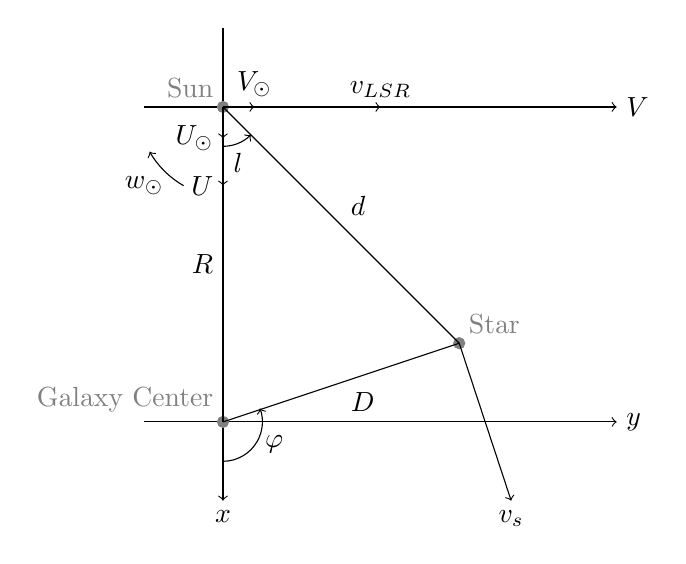
\begin{tikzpicture}
        % Axes
        \draw[->] (0,1) -- (0,-1) node[below, left] {$U$};
        \draw[->] (-1,0) -- (5, 0) node[right] {$V$};
        \draw[->] (-1, -4) -- (5,-4) node[right] {$y$};
        \draw[->] (0,-4) -- (0,-5) node[below] {$x$};

        % Points
        \filldraw [gray] (0,0) circle (2pt) node[above left] {Sun};
        \filldraw [gray] (0,-4) circle (2pt) node[above left] {Galaxy Center};
        \filldraw [gray] (3,-3) circle (2pt) node[above right] {Star};

        % Distances
        \draw (0,0) -- (3, -3) node[midway, above right] {$d$};
        \draw (0,-4) -- (3, -3) node[midway, below right] {$D$};
        \draw (0,0) -- (0, -4) node[midway, left] {$R$};

        % Relevant angles
        \draw[->] (0, -0.5) arc (-90:-45:0.5) node[midway, below] {$l$};
        \draw[->] (0, -4.5) arc (-90:20:0.5) node[midway, right] {$\varphi$};

        % Velocities
        \draw[->] (0,0) -- (2,0) node[right, above] {$\bm{v}_{\text{LSR}}$};
        \draw[->] (0,0) -- (0.4,0) node[right, above] {$\bm{V}_{\odot}$};
        \draw[->] (0,0) -- (0,-0.4) node[below, left] {$\bm{U}_{\odot}$};

        \draw[->] (3, -3) -- (3.66, -5) node[right, below] {$\bm{v_{\text{s}}}$};

        % rotational velocity of the sun around itself
        \draw[->] (-0.5, -1) arc (-120:-150:1.18);
        \draw node at (-1, -1) {$w_{\odot}$}; 

    \end{tikzpicture}
    \captionof{figure}{Frames of reference. The angular frequency $w_{\odot}$ only contributes to the tangential component of the velocities of the stars with in the Sun's frame of reference, and is therefore omitted in equation \ref{eq:ReferenceFrame}.}
    \label{fig:FrameOfReference}
\end{Figure}